\documentclass[openany]{book}

\usepackage{generalsnips}
\usepackage{calculussnips}
\usepackage[margin = 1in]{geometry}
\usepackage{pdfpages}
\usepackage[spanish]{babel}
\usepackage{amsmath}
\usepackage{amsthm}
\usepackage[utf8]{inputenc}
\usepackage{titlesec}
\usepackage{xpatch}
\usepackage{fancyhdr}
\usepackage{tikz}
\usepackage{hyperref}
\usepackage{cancel}
\usepackage{float}
\usepackage{amsfonts}
\title{Ecuaciones Diferenciales}
\date{2021 Enero 11} % , 09:57AM
\author{David Corzo}

\pagestyle{plain}
\definecolor{idedark}{rgb}{0.13,0.13,0.13}
\pagecolor{idedark}
\color{white}

\begin{document}
\maketitle
\tableofcontents
%%%%%%%%%%%%%%%%%%%%%%%%%%%%%%%%%%%%%%%%%%%%%%%%%%%%%%%%%%%%%%%%%%%%%%%%%%%%%%%%%%%%%%%%%%%%%%%%%%%%%%%%%%%%%%%%%%%%%%%%%%%%%%%%%%%%%%%%%%%%%%

\chapter{Introducción a las EDs}
\section{Introducción a las ecuaciones diferenciales}
\begin{itemize}
    \item Def: una ecuacion diferencial (ED) es una ecuación que contiene derivadas de una variable dependiente, generalmente $y$, respecto a una o más variables independientes, generalmente $x$ o $t$.
    \item Ejemplo: 
        \begin{itemize}
            \item crecimiento exponencial.
                \[
                    \dervpar{y}{t} = ky \qimplies y=f(t)?
                \]
            
            \item Enfriamiento de Newton:
                \[
                  \dervpar{T}{t} = K(T-T_m) \qimplies T?
                \]
            
            \item Deslizamiento: 
                \[
                  ay''+by'+cy'=f(t) 
                \]
            
            \item Logística: 
                \[
                  y'=Ky(M-y)
                \]
        \end{itemize}
    
    \item Objetivo: Encuentre una funcion $y(t)$ que satisfaga la ED.
\end{itemize}

\subsection{Definiciones}
\begin{itemize}
    \item ED Ordinaria: la ec tiene derivadas respecto a una \textbf{sola} variable.
    \item Ejemplo de ED ordinaria: 
        \[
          y'''+zy''+y'+y=x^3
        \]
    
    \item ED parcial: la ec tiene derivadas parciales respecto a dos o más variables.
    \item Ejemplo de ED parcial: ec de calor.
            \[
                \dervpar{u}{t} = \frac{\delta^2u}{\delta x^2} + \frac{\delta^2 u}{\delta y^2} 
            \]
\end{itemize}

\subsection{Orden de una ED}
\begin{itemize}
    \item el orden de la mayor derivada en la ED.
    \item ED orden 3: 
        \[
          \frac{d ^3y}{d x^3} + \p{\frac{d y}{d x} } ^4=\sin\p{ x } 
        \]
\end{itemize}

\subsection{Ejercicios}
Clasifique el orden de cada ED:
\begin{enumerate}
    \item ED 1er orden.
        \[
          \frac{d y}{d x} = Kx^2y^2
        \]
    
    \item ED 2do grado.
        \[
            p''=zpp'
        \]
    
    \item ED 3er orden.
        \[
          y'y'''+2y''+\alpha y' + \beta y = \sin\p{ x } e^{-2x}
        \]
    
    \item ED 2do orden.
        \[
            y(y'')^6+5(y')^20=0
        \]
\end{enumerate}

\subsection{Notaciones}
\begin{itemize}
    \item Notación prima: $\displaystyle y',y'',y^{(n)}$
    \item Notación Leibni: $\displaystyle \frac{d y}{d t} , \frac{d ^2y}{d t^2} , ... , \frac{d ^ny}{d t^n} $
\end{itemize}

\subsection{Forma de una ED}
\begin{itemize}
    \item ED de orden n: ponga las derivadas como variables.
        \[
          F(x, y,y',y'',...,y^{(n)}) = 0 \qq \text{ encuentre ¿y? }
        \]
    
    \item ED en su forma normal o estádar.
        \begin{itemize}
            \item Sólo la derivada más grande se encuentra en el lado izquierdo.
        \end{itemize}
        \[
            y^{(n)}=g(x,y,y',...,y^{(n-1)})
        \]
\end{itemize}

\subsection{Solución de una ED}
\begin{itemize}
    \item Solución: una funcion $y=\phi(x)$ que tiene $n$ derivadas continuas y satisface la ecuación diferencial.
    \item La idea es meter la función $y=\phi(x)$ en la ED y solucionarla.
\end{itemize}

\subsection{Ejercicio 2}
Verifique que $y(t)$ es una solución de la ED dada.
\begin{itemize}
    \item $\displaystyle \frac{d y}{d t} + 20y=24$. Solución: $\displaystyle y(t)=\frac{6}{5} -\frac{6}{5}e^{-20t}$. 
        \begin{center}
           \begin{align*}
               \text{ Derivar la solución: } \\ 
               y'(t) = +\frac{6}{5}\cdot 20e^{-20t} \\ 
               \text{ Remplaze $y'$ y $y$ en la ED. } \\ 
               \cancel{24e^{-20t}}+24-\cancel{24e^{-20t}} = 0 \\ 
               24e^{-20t}+20\p{\frac{6}{5}-\frac{6}{5}e^{-20t}} = 24 \\ 
           \end{align*}
        \end{center}
    
    \item $\displaystyle y''+4t=0$. Solución: $\displaystyle y(t) = c_1\cos\p{ 2t } +c_2\sin\p{ 2t } $ $c_1,c_2$ son constantes.
        \begin{center}
           \begin{align*}
               \text{ Derivamos dos veces (por el orden) la solución.} \\ 
               y'=-2c_1\sin\p{ 2t } + 2c_2\cos\p{ 2t } \\ 
               y''=-4c_1\cos\p{ 2t } -4c_2\sin\p{ 2t } \\ 
               \text{ Sustituir la segunda derivada en el problema original. } \\ 
               4c_1\cos\p{ 2t } -4c_2\sin\p{ 2t } +4\p{c_1\cos\p{ 2t } } + c_2\sin\p{ 2t } = 0 \\ 
               \cancel{4c_1\cos\p{ 2t }} - \cancel{4c_2\sin\p{ 2t }} +\cancel{4\p{c_1\cos\p{ 2t } }} + \cancel{c_2\sin\p{ 2t }} = 0 \\ 
               0 = 0 \qq \text{ $y(t)$ es la soln de la ED. } \\ 
           \end{align*}
        \end{center}
\end{itemize}

\subsection{Soluciones triviales}
\begin{itemize}
    \item Soln trivial: una ED tiene soln trivial si la función cero $\phi(x)=0$ es una de sus soluciones.
    \item Ejemplo de no tener solucion trivial:
        \begin{center}
           \begin{align*}
               y'+20y=24 \\ 
               y = 0, \qq y'=0 qq 0+20\cdot 0 = 0 \neq 24 \\ 
           \end{align*}
        \end{center}
    
    \item Ejempo de tener solución trivial:
        \begin{center}
           \begin{align*}
               y''+4y=0 \\ 
               y = y'' = 0 \qq 0+4\cdot 0 = 0 = 0 \\ 
           \end{align*}
        \end{center}
\end{itemize}

\subsection{Infinitas soluciones}
\begin{itemize}
    \item Una ED puede tener infinitas soluciones.
    \item Considere la ED: $\displaystyle \frac{d y}{d x} = f(x)$.
        \begin{itemize}
            \item La integral de $y'$: 
                \begin{center}
                   \begin{align*}
                        \int \frac{d y}{d x} dx = \int f(x) dx \\ 
                        y = \int_{}^{}f(x) dx = F(x) + C \\ 
                   \end{align*}
                \end{center}
            \item $y'$ dependiente. $x$ independiente
            \item La solución de esta ED es la antiderivada de $f(x)$ .
            \item Hay infinitas soluciones: $y = F(x) + C$ 
            \item La familia de soluciones de la ED es: $F(x)+C$.
            \item Entonces necesitamos encontrar el valor de $C$.
        \end{itemize}
        \begin{figure}[H]
            \centering
            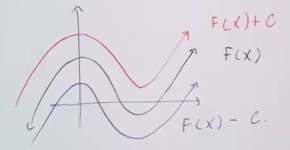
\includegraphics[width=0.4\textwidth]{./Figs/2021-01-11-10-50-53.png}
        % 	\caption{}
        \end{figure}
        \begin{itemize}
            \item No sólo se encuentra $F(x)$ sino también el calor de $C$.
        \end{itemize}
\end{itemize}

\subsection{2 tipos de soluciones para una ED}
\begin{itemize}
    \item La solución general: la solución contiene constantes arbitrarias $c_1,c_2,...,c_n$. (infinitas soluciones)
    \item La solución particular: la solución no contiene constantes arbitrarias. (solución unica)
\end{itemize}

\subsection{Ejemplo}
\begin{enumerate}
    \item $\displaystyle \frac{d y}{d t} + 20y=24$ 
        \begin{center}
           \begin{align*}
               y(t) = \frac{6}{5}+\frac{6}{5}e^{-20t} \\ 
               \text{ Solución particular de la ED. } \\ 
           \end{align*}
        \end{center}
    
    \item $\displaystyle \frac{d ^2y}{d t^2}+4y=0 $ 
        \begin{center}
           \begin{align*}
               y(t) = c_1\cos\p{ 2t } +c_2\sin\p{ 2t } \\ 
               \text{ Solución general. } \\ 
           \end{align*}
        \end{center}
\end{enumerate}

\subsection{Hay una correlación directa entre el orden de la ED y el número de constantes arbitrarias que resultan de la integración}
\begin{itemize}
    \item En general la solución general de una ED depende del orden de la ecuación diferencial.
    \item ED 1er orden: 1 constante arbitraria.
    \item ED 2do orden: 2 constantes arbitraria.
    \item ED n-ésimo orden: n constantes arbitrarias.
\end{itemize}

\subsection{Resolver el siguiente ejercicio}
\begin{itemize}
    \item $\displaystyle \frac{d y}{d t} +20y=24$ 
        \begin{center}
           \begin{align*}
               \frac{d y}{d t} = 24 - 20y \\ 
               \underbrace{\int_{}^{} \frac{dy}{24-20y} = \int_{}^{}dt}_{\text{ Recordar: } \int_{}^{}\frac{d y}{y + b} } = \ln|y+b|+C   \\ 
               -\frac{1}{20}\ln\p{ 24-20y } = t + C \qimplies \text{ ya no hay derivadas entre y } \\
               24-20y = e^{-20t-20C} \\ 
               -20y = -24 - e^{-20t-20C} \\ 
               y = \frac{6}{5}+\frac{1}{20}e^{-20t-20C} \\  
               \text{ Tenemos una solución general, nos deben dar una condición inicial para sacar la solución particular. } \\ 
           \end{align*}
        \end{center}
\end{itemize}


\chapter{Problemas de valor inicial}
\begin{itemize}
    \item EDs 1er orden:
        \[
          \frac{d y}{d x} = f(x,y) = e^x\sin\p{ y } 
        \]
    
    \item Solución general: 
        \[
          \phi(x,y)+C
        \]
    \item Solución particular: son libres de constantes.
\end{itemize}
Son necesarias condiciones en la variable $y(x_0)=y_0$  y sus derivadas para no tener constantes arbitrarias.

\subsection{Problema de valor inicial (PVI) de primer orden}
\begin{itemize}
    \item Es una ED de 1er orden con una condición inicial.
        \[
          \frac{d y}{d x} = f(x,y), \qq y(x_0) = y_0
        \]
\end{itemize} 

\subsection{PVI de 2do grado}
\[
  \frac{d ^2y}{d x^2} = f(x,y,y'), \qq y(x_0)=y_0 11 y'(x_0)=V_0
\]
En física, tienen la aceleración $y''$ $y$ quieren encontrar el desplazamiento. Se necesita la posición inicial $y(0)=y_0$ y la velocidad inicial $y'(0)=V_0$.

\subsection{Ejercicio 1: Encuentre la solución particular de las sigs EDs.}
\begin{itemize}
    \item $\displaystyle y'=y-y^2$, $\displaystyle y(-1)=5$ Use la solución general: $\displaystyle y(x)=\frac{1}{1+ce^{-x}}$ 
        \begin{itemize}
            \item Recordar que lo único que tenemos que hacer es encontrar la constante de la solución general.
        \end{itemize}
        \begin{center}
           \begin{align*}
               \text{ Use: } \qq x=-1, \qq y=5 \qq \text{ para encontrar el valor de C. } \\ 
               \frac{1}{1+ce^1}=5 \qimplies 1+ce^1=\frac{1}{5} \\ 
               ce=\frac{1}{5}-1 \qimplies  c= -\frac{4}{5e} \\ 
               \text{ Solución particular: } \qq y(x)=\frac{1}{1-\frac{4}{5e}e^{-x}} \\ 
           \end{align*}
        \end{center}
    
    \item $\displaystyle u''+u=0, \qq u(\pi/2)=2, \qq u'(\pi/2)=5$ Use la solución general $\displaystyle u = c_1\sin\p{ x } +c_2\cos\p{ x } $.
        \begin{center}
           \begin{align*}
               u' = c_1\cos\p{ x } -c_2\sin\p{ x } \\ 
               \text{ Aplique cada una de las CIs. } \\ 
               u(\pi/2) = c_1\cdot 1 + c_2\cdot 0 \qimplies  c_1 = 2 \\ 
               u'(\pi/2) = c_1\cdot 0 - c_2\cdot 1 = 5 \qimplies c_2 = -5 \\ 
               \text{ Solución particular: } u(x) = 2\sin\p{ x } -5\cos\p{ x } \\ 
           \end{align*}
        \end{center}
\end{itemize}


\subsection{Resolución de una ED}
Casos:
\begin{enumerate}
    \item Solución única.
    \item Infinitas soluciones.
    \item No hay solución, ocurre en un PVI (usualmente cuando se ponen condiciones imposibles).
\end{enumerate}

\begin{itemize}
    \item No todos los problemas con valor inicial con condiciones tienen soluciones únicas.
    \item Por ejemplo: $\displaystyle \frac{d y}{d t} =3y^{2/3}$  sujera a $y(0)=0$ tiene por lo menos 2 soluciones. $y(t)=0 \qq y(t)=t^3$.
        \begin{itemize}
            \item ¿Cómo sabemos que es $t^3$?
                \begin{center}
                   \begin{align*}
                       \frac{dy}{3y^{2/3}}=dt \qq \text{ integrar. } \\ 
                        \int_{}^{}\frac{1}{3}y^{-2/3}dy = \int_{}^{}dt \\ 
                        \frac{3}{3}y^{1/3} = t + c \\ 
                        y = (t+c)^3 \qq \text{ Solución general } \\ 
                        0 = (0 + c)^3 \qimplies c^3=0 \qimplies c=0 \\ 
                        \text{ Solución particular: } \qq y = t^3 \\ 
                   \end{align*}
                \end{center}
        \end{itemize}
\end{itemize}

\subsection{¿Cuándo un PVI tiene garantizada solución única?}
\begin{itemize}
    \item El problema de valor inicial de primer orden $y'=f(x,y)$ $y(x_0)=y_0$ tiene garantizada una solución única si $f(x,y)$ y $\frac{\delta f}{\delta y} $ son continuas en $(x_0,y_0)$.
\end{itemize}

\subsection{Ejercicios}
Ejercicio 2a: Encuentre y grafique los puntos $(x,y)$ donde la solución única del PVI está garantizada.
\begin{itemize}
    \item $\displaystyle y'=y-y^2$ 
        \begin{center}
           \begin{align*}
               f(x,y)=y-y^2 \qq \text{ es continua en } \qq \mathbb{R^2} \\ 
               \frac{\delta f}{\delta y} = 1-2y \qq \text{ es continua en } \qq \mathbb{R^2} \qq \text{(plano)} \\ 
               \text{ La solución única está garantizada en: } \qq -\infty<x<\infty \qq -\infty<y<\infty \\ 
           \end{align*}
           \begin{figure}[H]
               \centering
               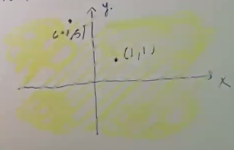
\includegraphics[width=0.4\textwidth]{./Figs/2021-01-13-10-35-55.png}
           % 	\caption{}
           \end{figure}
        \end{center}
    
    \item $\displaystyle y'=3y^{2/3}$ 
        \begin{center}
           \begin{align*}
               f(x,y)=3y^{2/3} \qq \text{ es continua en $\mathbb{R}^2$ } \\ 
               \text{ Pero: } \qq \frac{\delta f}{\delta y} = \frac{3\cdot 2}{3}y^{-1/3} = \frac{2}{y^{1/3}} \\ 
               \text{ No es continua en $y=0$. No hay solución garantizada si $y=0$ $(x,y), y\neq 0$. } \\ 
           \end{align*}
        \end{center}
    
    \item $\displaystyle y'=\frac{\sqrt{y^4-16}}{x}$ 
        \begin{itemize}
            \item Evite números negativos.
            \item Evite denominador igual a cero.
        \end{itemize}
        \begin{center}
           \begin{align*}
               f(x,y) = \frac{\sqrt{y^4-16}}{x} \qq \text{ no es continua en x=0 \& -2<y<2 } \\ 
               y^4-16 \geq 0 \qimplies y^4 \geq 16 \qimplies -2\geq y \geq 2 \\ 
               \text{ Adicionalmente: } \frac{\delta f}{\delta y} = \frac{1}{x}(y^4-16)^{-1/2} \frac{1}{2}4y^3 \\ 
               \frac{\partial f}{\partial y} = \frac{2y^3}{x\sqrt{y^4-16}} \qq \text{ se indefine en: }\qq \pm 2 \\ 
               \text{ Solución garantizada si } \qq x=0 \qq -2\leq y \leq2 \\ 
           \end{align*}
           \begin{figure}[H]
               \centering
               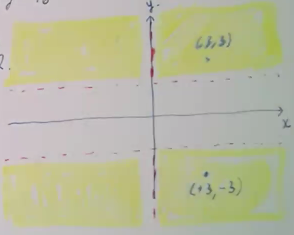
\includegraphics[width=0.4\textwidth]{./Figs/2021-01-13-10-47-35.png}
           % 	\caption{}
           \end{figure}
        \end{center}
\end{itemize}

\subsection{ED separable de primer orden}
\[
  \frac{d y}{d x} = f(x)g(y)
\]
\begin{itemize}
    \item el lado derecho es un producto de dos funciones en $x$ y en $y$.
    \item ED lineal de 1er orden.
        \[
          a(x)\frac{d y}{d x} + b(x)y = c(x)
        \]
    
    \item Las funciones coeficientes $a,b,c$ sólo dependen de x.
        \[
          \frac{d y}{d x} \qq \text{ \& } \qq y \qq \text{ sólo tienen potencias de uno. }
        \]
    
    \item ED exacta:
        \[
          M dy + N dx = 0  \qq \frac{\partial M}{\partial x} = \frac{\partial N}{\partial y} \\ 
        \]
    
    \item Una ED de 1er orden $\displaystyle \frac{d y}{d x} = f(x,y)$ se puede escribir usando diferenciales. La idea es tratar el $dy,dx$ como una fracción.
        \[
          dy=f(x,y)dx \qimplies dy=f(x,y)dx=0
        \]
\end{itemize}

\subsection{Ejercicio 3}
Determine si la ED dada es lineal o es separable.
\begin{enumerate}
    \item $\displaystyle (y-x^2)dx+4ydy = 0$
        \begin{center}
           \begin{align*}
               (y-x^2)dx+4xdy = 0 \\ 
               (y-x^2)+4x\frac{d y}{d x} =0 \\ 
               4x\frac{d y}{d x} = x^2-y \\ 
               \frac{d y}{d x} = \frac{x^2-y}{4x} \qimplies \text{ No es separable por el término $x^2-y$} \\ 
           \end{align*}
           \begin{itemize}
               \item Pero sí es lineal.
           \end{itemize}
           \begin{align*}
                4x\frac{d y}{d x}  + y = x^2 \\ 
                a(x) = 4x, \qq b(x) = 1, c(x) = x^2 \\ 
           \end{align*}
        \end{center}
    
    \item $\displaystyle ydx+(x+xy+e^y)dy=0$ 
        \begin{center}
           \begin{align*}
               y + \underbrace{(x+xy+e^y)}_{a(x)}\frac{d y}{d x} = 0 \qq \text{ No es lineal. } \\ 
               (x+xy+e^y)\frac{d y}{d x} = -y
               \frac{d y}{d x} = \frac{-y}{(x+xy+e^y)} \qq \text{ No es separable. } \\ 
           \end{align*}
        \end{center}
    
    \item $\displaystyle ydx+(xxye^y)dy=0$ 
        \begin{center}
           \begin{align*}
               x^2ye^y\frac{d y}{d x} +y = 0 \qq \text{ No es lineal. } \\ 
               \frac{d y}{d x} = \frac{-y}{x^2ye^y} = -\frac{1}{x^2e^y} = \p{-\frac{1}{x^2}} \p{\frac{1}{e^y}} \qq \text{ Es separable. } \\ 
               \text{ Separe en términos de $x$ \& de $y$. } \\ 
               e^ydy=-\frac{1}{x^2}dx \\ 
               \int e^ydy=\int -x^{-2}dx \\ 
               e^y + c_1 = x^{-1} + c_2 \\ 
               y = \ln\p{ c_2 - c_1 + \frac{1}{x} } \qimplies \text{ Solución general. } \\ 
           \end{align*}
        \end{center}
\end{enumerate}


\chapter{Ecuaciones diferenciales 1er orden separables}
\section{Ecuaciones diferenciales Separables}
\begin{itemize}
    \item ED de 1er grado separable: es una ED de 1er grado cuyo lado derecho es un producto de una función en $x$ y una función $y$.
        \[
          \frac{d y}{d x} = f(x)g(y) \qq \text{ o } \qq g(y)dy+f(x)dx=0
        \]
    
    \item Resolución: se coloca cada variable en un lado de la ecuación y se integra respecto a cada variable. Ya con eso eliminamos la derivada, pero debemos resolver para $y$.
        \begin{center}
           \begin{align*}
               \frac{d y}{g(y)} = f(x)dx \qimplies \int \frac{d y}{g(y)} = \int f(x)dx \\ 
               G(y) = F(x) + C \\ 
               \text{ Las dos constantes de integración se pueden combinar en una sola $C = C_2-C_1$  } \\ 
           \end{align*}
        \end{center}
    
    \item Ejemplos: 
        \begin{center}
           \begin{align*}
               \frac{d y}{d x} = y^3x^2e^{x^3+y^4} = (y^3e^{y^4})(x^2e^{x^3}) \qimplies \text{ Separable. } \\ 
               \frac{d y}{d x} = tan(y+x) \qimplies \text{ No es separable. } \\ 
           \end{align*}
        \end{center}
\end{itemize}

\subsection{Ejercicio 1: Resuelva}
Pasos:
\begin{enumerate}
    \item Separe.
    \item Integre.
    \item Resuelva para $y$.
\end{enumerate}
\begin{enumerate}
    \item $\displaystyle \frac{d y}{d x} = -3x^2y^2$ 
        \begin{center}
           \begin{align*}
                \frac{d y}{d x} = -3x^2y^2 \qq \text{ Como un cociente de diferenciales $\frac{d y}{d x} $ }. \\ 
                \frac{d y}{-y^2} = 3x^2dx \qq \text{ Separe. } \\ 
                \int -y^{-2}dy = \int 3x^2dx \qq \text{ Integre. } \\ 
                \frac{1}{y}=x^3+C \qq \text{ Resuelva para $y$ } \\ 
                y = \frac{1}{x^3+C} \\ 
           \end{align*}
        \end{center}
        \begin{itemize}
            \item $\displaystyle \frac{d y}{d x} =f(x)$ también es ED separable porque $g(x)=1$.
                \begin{center}
                    \begin{align*}
                        \int dy = \int f(x) dx \qimplies y = F(x) + C \\ 
                    \end{align*}
                \end{center}
        \end{itemize}
    
    \item $\displaystyle \frac{d y}{d x} =\frac{1}{\sqrt{1-x^2}}$ 
        \begin{center}
           \begin{align*}
                \frac{d y}{d x} =\frac{1}{\sqrt{1-x^2}} \qq \text{ Si es separable. } \\ 
                \int dy = \int \frac{dx}{\sqrt{1-x^2}} \\ 
                y = \arcsin\p{ x } + C \\ 
           \end{align*}
        \end{center}
\end{enumerate}

\subsection{Una ED puede tener una C.I. $y(a)=b$}
\begin{enumerate}
    \item $\displaystyle \frac{d y}{d x} = y^2\sec\p{ x } \tan\p{ x } $ $y(0)=0.5$
        \begin{itemize}
            \item Tomar en cuenta que esta ED no es lineal por el término $y^2$.
        \end{itemize}
        \begin{center}
           \begin{align*}
               \text{ Separe:  } &\qq \frac{d y}{y^2} = \sec\p{ x } \tan\p{ x } dx \\ 
               \text{ Integre: } &\qq \int y^{-2} dy = \int \sec\p{ x } \tan\p{ x } dx  \\ 
               &\qq \frac{1}{y}= \sec\p{ x } + C \\ 
               \text{ Resuelva para y: } &\qq \frac{-1}{\sec\p{ x } +C} = y \qq \text{ Sol. General. } \\ 
               \text{ Use $y(0)=0.5$ para encontrar c, $sec(0)=1$   } \\ 
               0.5=\frac{-1}{\sec\p{ 0 } +C} \qimplies -0.5 = \frac{1}{1+C}  \\ 
               1+C = \frac{1}{-0.5}=-2 \\ 
               C = -2-1 = -3 \\ 
               \text{ Soln: } \qq y = \frac{-1}{\sec\p{ x } -3} \\ 
           \end{align*}
           \begin{itemize}
               \item Pueden encontrar C, antes de resolver para $y$ también.
           \end{itemize}
           \begin{align*}
               -\frac{1}{y}= \sec\p{ x } + C \qq x=0, y =0.5 \\ 
            -\frac{1}{0.5} = 1+C \\ 
            -\frac{1}{y}= \sec\p{ x } -3 \qimplies -\frac{1}{\sec\p{ x } -3} = y \\             
           \end{align*}
        \end{center}
    
    \item $\displaystyle \frac{d y}{d x} = -\frac{y}{x^2}$ $y(1)=e^2$ 
        \begin{itemize}
            \item El PVI no tiene solución única en $x=0$, se indefine en 0.
            \item Sí hay solución única en (1,1).
        \end{itemize}
        \begin{center}
           \begin{align*}
               \int \frac{d y}{y}  = \int -\frac{d x}{x^2} \\ 
               \ln\p{ y } = \frac{1}{x} + C \qq \text{ Use $x=1, y=e^2$  }\\ 
               C = \ln\p{ y } - \frac{1}{x} \\
               C = \ln\p{ y } - \frac{1}{x} = \ln\p{ e^2 } - \frac{1}{1} = 2 -1 = 1 \\ 
               \ln\p{ y } = x^{-1} + 1 \qq \text{ use $e^{\ln\p{ [] }  }$ = [] }   \\ 
               y = e^{x^{-1}} = e^{1+\frac{1}{x}} \\ 
               \text{ Solución general: } y = e^{1/x+C} \\ 
           \end{align*}
        \end{center}
        \begin{itemize}
            \item Esto se puede ver como una 'integración implícita'.
            \item Solución implícita: la solución de una ED separable es una función implícita.
                \[
                  G(y) = F(x)+C \qimplies \text{ Explicita: } \qq y = H(x) + C 
                \]
                En algunos casos no es posible resolver para y. Por ejemplo el siguiente.
        \end{itemize}
    
    \item $\displaystyle \frac{d y}{d x} = \frac{4x}{1+y+y^2}$
        \begin{center}
           \begin{align*}
               \int (1+y+y^2)dy = \int 4xdx \\ 
               y + 0.5y^2 + \frac{1}{3}y^3 = 2x^2 + C \\ 
           \end{align*}
           \begin{itemize}
               \item No se puede resolver para $y$, la solución es la función implícita.
                \[
                  y + 0.5y^2 + \frac{1}{3}y^3  -x^2 = 15 
                \]
           \end{itemize}
        \end{center}
\end{enumerate}

En algunas EDs separables es necesario realizar fracciones parciales.
\begin{enumerate}
    \item Resuelva: $\displaystyle \frac{d y}{d x} = y^2-9$
        \begin{center}
           \begin{align*}
               \int \frac{dy}{y^2-9} = \int dx = x+c \qq \text{ Se debe hacer fracciones parciales. } \\ 
                \text{ Encuentre las fracciones parciales: } \\ 
                \frac{1}{y^2-9} = \frac{1}{(y-3)(y+3)} = \frac{A}{y-3}+ \frac{B}{y+3} \\ 
                \text{ Multiplique por:  } \qq (y-3)(y+3) \\ 
                y = 3: \qimplies  A(y+3) + B(y-3) = 1 \\ 
                y = -3: \qimplies  6A + 0 = 1 \qimplies A = \frac{1}{6} \\ 
                0 - 6B = 1 \qimplies B=-\frac{1}{6} \\ 
                \text{ Integre la variable $y$ } \\ 
                \frac{1}{6}\int \frac{dy}{y-3} - \frac{1}{6}\int \frac{dy}{y+3} = x+c \\ 
                \frac{1}{6}\p{\ln\p{ y-3 } - \ln\p{ y+3 }  } = x+c \\ 
                \ln\p{ y-3 } -\ln\p{ y+3 } = 6x+6c \\ 
                \ln\p{ \frac{y-3}{y+3} } = 6x + 6c \\ 
                \frac{y-3}{y+3} = e^{6x + 6c} \\ 
                y-3 = ye^{6x+6c}+ 33^{6x+6c} \\ 
                y\p{1-e^{6x+6c}} = 3+3e^{6x+6c} \\ 
                y = 3+3e^{6x+6c} \qq \text{ Solución general. } \\ 
           \end{align*}
           \begin{figure}[H]
               \centering
               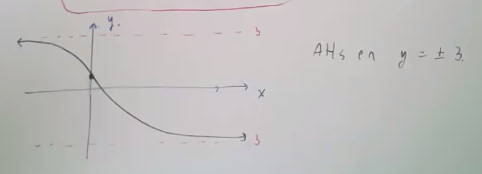
\includegraphics[width=0.8\textwidth]{./Figs/2021-01-18-10-58-09.png}
           % 	\caption{}
           \end{figure}
        \end{center}
    
    \item Integre: $\displaystyle \int \frac{y-2}{y^2-9}$ 
        \begin{center}
           \begin{align*}
               \frac{y-2}{(y-3)(y+3)} = \frac{A}{y-3} + \frac{B}{y+3} \\ 
               y-2 = A(y+3)+B(y-3) \\ 
                y=3: \qq  1 = 6A \qimplies A = 1/6 \\ 
                y =-3: \qq -5 = -6B \qimplies B = 5/6 \\ 
                \frac{A}{y-3} + \frac{B}{y+3} = \frac{1}{6}\ln\p{ y-3 } + \frac{5}{6}\ln\p{ y+3 } +c \\  
                \text{ La ED } \qq  \frac{d y}{d x} =y^2-9 \qimplies y^2-9=0 \qq \text{ cuando: } \qq y \pm 3 \\ 
                \text{ Tiene otras dos soluciones $y = \pm 3$ contantes.} \\ 
                \text{ Solución general:  } \qq y = 3(1+e^{6x+6c}) \\ 
                \text{ Las soluciones $y\pm 3$ se conocen como soluciones singulares: } \\ 
                \text{ Porque:  } \qq \int \frac{dy}{y^2-9} \qq \text{ se indefine en  } \qq x\pm 3 \\ 
           \end{align*}
        \end{center}
\end{enumerate}

Solución singular:
\begin{itemize}
    \item La ED $\displaystyle \frac{dy}{dx}=g(x)h(y)$  tiene soluciones cuando $h(y)=0$.
    \item Solución singular de una ED: son las soluciones $y=c$  donde $h(c)$ 
\end{itemize}


\chapter{Ecuaciones diferenciales lineales}
\section{ED lineales}
\begin{itemize}
    \item ED lineal 2do orden: 
        \[
          A(X)y''+B(x)y'+C(x)y=D(x)
        \]
    
    \item ED lineal 1er orden:
        \[
          A(x)y'+B(x)y=C(x)
        \]
    
    \item En general no es separable $\displaystyle C(x) -B(x)y$.
    \item Divida la ED lineal por $\displaystyle A(x)$ para obtener su forma estándar.
        \[
          y'+P(x)y=Q(x)\qq, P=\frac{B}{A}\qq, Q=\frac{C}{A}
        \]
\end{itemize}


\subsection{Resolución de una ED lineal}
\begin{center}
    \begin{align*}
        Q(x)=0 \qq \text{ Resuelva } \qq \frac{d y}{d x} = P(x)y \qq \text{ separable. } \\ 
        \int \frac{d y}{y} = \int P(x)dx \qimplies \ln\p{ y } =\int P(x)dx \qimplies y=e^{\int P(x)dx} \\ 
        y' = e^{\int P(x)dx} \cdot P(x) \qq \text{ Usar el teorema fundamental del cálculo: } \qq \frac{d }{d x} \int P dx = \int P(x) dx =P \\ 
    \end{align*}
\end{center}
\begin{enumerate}
    \item Factor de integración $\displaystyle v=e^{\int P(x)dx}$ 
    \item Multiplique la ED por el factor de integración:
        \[
            y'e^{\int P dx} + y P(x) e^{\int P dx} = Q(x)e^{\int P(x)dx}
        \]
        \begin{itemize}
            \item Recordar regla del producto $\displaystyle u\cdot v = u'v + uv'$.
        \end{itemize}
        \begin{center}
            \begin{align*}
                \p{ye^{\int P(x)dx}}' = y'e^{\int P dx}  + yP(x)e^{\int P dx} \\ 
            \end{align*}
        \end{center}
    
    \item Use la regla del producto en ``reversa'':
        \begin{center}
           \begin{align*}
               \frac{d }{d x} \p{ye^{\int P sx}} = Q(x)e^{\int P dx} \\ 
           \end{align*}
        \end{center}
    
    \item Integre ambos lados de la ec:
        \begin{center}
           \begin{align*}
               y e^{\int P dx} = \int Q(x)e^{\int Pdx} + C \\ 
           \end{align*}
        \end{center}
    
    \item Resuelva para $y$:
        \[
          y = e^{-\int Pdx}\int Q(x)e^{\int Pdx}dx + ce^{-\int Pdx} 
        \]
\end{enumerate}

\subsection{Pasos ED lineal}
\begin{itemize}
    \item Verifique que la ED es lineal.
    \item Escriba la ED en su forma estándar.
    \item Factor de integración $\displaystyle e^{\int P(x)dx}$.
    \item Multiplique la ecuación diferencial $\times$ factor de integración.
    \item Utilice la regla del producto.
    \item Integre la ED y resuelva para $y$.
\end{itemize}


\subsection{Ejercicios}
\begin{enumerate}
    \item $\displaystyle y'+2xy=4x$  es lineal y es estándar.
        \begin{center}
           \begin{align*}
               \text{ Factor de integración: } &\qq e^{\int Pdx} = e^{\int 2xdx} = e^{x^2} \qq \text{ Agregaremos C al final } \\
               \text{ Multiplique la ED por el FI: } &\qq y'\p{e^{x^2}}  + y\p{2xe^{x^2}}  = 4xe^{x^2} \\ 
               \text{ Utilice la regla del producto en reversa: } &\qq \p{ye^{x^2}}' = 4xe^{x^2} \\ 
               \text{ Integre ambos lados respect a $x$: } &\qq \int\p{ye^{x^2}}'dx = \int 4xe^{x^2} dx \qimplies 2e^{x^2}+C \\ 
               &\qq u = x^2, \qq du = 2xdx \qimplies \int 2e^udu=2e^u \\ 
               \text{ Resuelva para $y$: } \qq y = \frac{2e^{x^2}+C}{e^{x^2}} = 2+Ce^{-x^2} \\ \text{ También es separable } \qq y'=4x-2xy=2x(2-y) \\ 
                \int \frac{dy}{2-y}=\int 2x dx \qimplies -\ln\p{ 2-y } =x^2-C \\ 2-y=e^{-x^2-c} \qimplies 2-e^{-x^2-c} = y \qimplies c_1 = -e^{-c} \\ 
           \end{align*}
        \end{center}
    
    \item $\displaystyle 2\p{y-4x^2} dx+xdy=0$ no es separable.
        \begin{center}
           \begin{align*}
               \text{ Rescriba la ED } &\qq 2y-8x^2+x \frac{d y}{d x} = 0 \\ 
               &\qq xy'+2y=8x^2 \qq \text{ ED lineal } \qq e^{2x} \\ 
               y'+\frac{2}{x}y  =8x \qq \text{ ED lineal estándar } \\ 
               \text{ FI }&\qq \int Pdx=\int \frac{2}{x}dx  = 2\ln\p{ x } \\ 
               &\qq 2x \neq e^{\int Pdx}  = e^{2\ln\p{ x } }= e^{\ln\p{ x^2 }  } = x^2 \\ 
               \text{ Multiplique por el FI } &\qq x^2y'+2xy=8x^3 \\ 
               &\qq \p{x^2y}' = 8x^3 \\ 
               \text{ Integre: } &\qq x^2y=\int 8x^3 dx \qimplies x^2y = 2x^4+C \\ 
               \text{ Sol general: } &\qq y = \frac{2x^4+C}{x^2} \qimplies 2x^2+Cx^{-2} \\ 
           \end{align*}
        \end{center}
    
    \item $\displaystyle \p{\cos\p{x} +2y\cos\p{ x } } dx -\sin\p{ dy } =0$ 
        \begin{center}
           \begin{align*}
               \p{\cos\p{ x } + 2y\cos\p{ x } } -\sin\p{ x } \frac{d y}{d x} =0 \\ 
               \cos\p{ x } = \sin\p{ x } \frac{d x}{d y} -2y\cos\p{ x } qq \text{ ED lineal } \\ 
               \frac{d y}{d x} -2\frac{\cos\p{x}}{\sin\p{ x } }y  = \frac{\cos\p{ x } }{\cos\p{ x } } \qq \text{ Forma estándar } \\ 
               \text{ FI } \qq -2\int \frac{\cos\p{ x } }{\sin\p{ x } }dx = \qq  \underbrace{-2\int \frac{du}{u} = }_{u=\sin\p{ x }, du=\cos\p{ x } dx} = -2\ln\p{ \sin\p{ x }  } \\ 
               \qq e^{\int P dx} = e^{-2\ln\p{ \sin\p{ x }  } } = e^{\ln\p{ \sin^{-2}\p{ x }  }  } \\ 
               \text{ Multiplique por el FI } \qq \frac{\sin^{-2}\p{ x }y' }{f_1} -2\frac{\cos(x)}{\sin^{3}(x)} \qimplies \int u^{-3}du = \frac{u^-2}{-2}+C \\ 
               \frac{y}{\sin^{2}(x)} = \int \sin^{-3}\p{ x } \cos\p{ x } dx  = -\frac{1}{2}\sin^{-2}\p{ x } +C \qimplies y = -0.5+C\sin^2(x) \\ 
           \end{align*}
        \end{center}
\end{enumerate}


\chapter{Ecuaciones diferenciales exactas}
\section{ED exactas}
\begin{itemize}
    \item Una ED de 1er orden que es $\displaystyle \frac{d y}{d x} = \frac{M(x,y)}{N(x,y)}$ (usualmente escritas en términos de sus diferenciales) se puede escribir en términos de sus diferenciales: $\displaystyle Mdx = Ndy \qimplies M(x,y)dx-N(x,y)dy = 0$.
    \item La ED exacta no siempre es separable o lineal.
    \item ED exactas: 
        \[
            \frac{\partial M}{\partial y} = \frac{\partial N}{\partial x} \\ 
        \]
    
    \item Solución de una ED exacta: Si la ED 1er orden $\displaystyle Mdx - Ndy = 0$ es exacta, entonces la solución de la ED satisface las siguientes ecuaciones:
        \[
          \frac{\partial F}{\partial x}  = M \qq \frac{\partial f}{\partial y} = N
        \]
        \begin{itemize}
            \item Solución general: la función implícita $F(x,y)=c$.
        \end{itemize}
    
    \item Pasos para resolver:
        \begin{itemize}
            \item Derivar de manera cruzada: ED exacta:
                \[
                  M_y = N_x
                \]
            
            \item Integre respecto a $x$:
                \[
                  F_x = M(x,y)
                \]
                \begin{itemize}
                    \item La constante depende de $y$.
                    \item Inicialmente uno tendrá una solución como $\displaystyle F+A(y)$ 
                \end{itemize}
            
            \item Derive $F$ respecto a $y$: $\displaystyle F_y+A'(y)=N$ 
                \begin{itemize}
                    \item Simplifique e integre $A'(y)$.
                \end{itemize}
            
            \item Solución general $\displaystyle F(x,y)=c$.
        \end{itemize}
\end{itemize}

\subsection{Ejercicio}
Resuelva las EDs.
\begin{enumerate}
    \item $\displaystyle \p{3x^2y-6x}dx + \p{x^3+2y}dy = 0$ 
        \begin{center}
           \begin{align*}
                \underbrace{\p{3x^2y-6x}}_{M}dx + \underbrace{\p{x^3+2y}}_{N}dy = 0 \\ 
                \frac{\partial M}{\partial y} = 3y^2 \qq \frac{\partial N}{\partial x} = 3x^2 \qq M_y = N_x \; \text{ Ed exacta }\\ 
                \text{ La ED satisface las condiciones   } \\ 
                \frac{\partial F}{\partial x} = 3x^2y-6x \qq \frac{\partial f}{\partial y} = x^3+2y \\ 
                \text{ Integre $F_x$: }\; F(x,y) = x^3y-3x^2+C(y) \\ 
                \text{ Derive $F$ respecto  $y$: } \; \frac{\partial F}{\partial y} = x^3+C'(y)=x^3+2y \\ 
                \text{ Simplifique e integre: }\; C'(y)=2y \qq C(y)=y^2 \\ 
                \text{ Solución general: }\; F=C \qq x^3y-3x^2+y^2=C \\                 
           \end{align*}
           \hlinefill
            \begin{align*}
            \text{ Puede empezar integrando la 2da ec: } \\ 
            F(x,y) = x^3y+y^2+A(x) \\ 
            F_x = 3x^2y+A'(x)=3x^2y-6x \\ 
            A'(x)=-6x \qimplies A(x = -3x^2) \\ 
            \text{ Misma solución general: }\; x^3y-3x^2+y^2=c \\ 
            \end{align*}
        \end{center}
    
    \item $\displaystyle (2x^3-xy^2-2y+3)dx-(x^2y+2x+2y)dy=0$
        \begin{center}
           \begin{align*}
               M_y = -2xy-2 \qq N_x = -2xy-2) \qq \text{ (es exacta) } \\ 
               F_x = 2x^3-xy^2-2y+3 \qq F_y=-x^2y-2x-2y \\ 
               \text{ Integre: }\; F=\frac{2}{4}x^4-\frac{1}{2}x^2y^2-2yx+3x +A(y) \\ 
                \text{ Derive: }\; F_y = -x^2y-2x+A'(y)=\cancel{-x^2y}-\cancel{2x}-2y \\ 
                \text{ Integre: }\; A'(y) = -2y \qimplies A(y)=-y^2 \\ 
                \text{ Soln. General: }\; \frac{1}{2}x^4 -\frac{1}{2}x^2y^2-2yx+3x-y^2=c \\ 
           \end{align*}
        \end{center}
    
    \item $\displaystyle (\cos\p{ x } \sin\p{ y } -\cot\p{ x } )dx - (\sec\p{ y } -\sin\p{ x } \sin\p{ y } )dy=0$ 
        % \begin{center}
        %    \begin{align*}
        %        M_y = -\cos{x} \sin\p{ y } 
        %    \end{align*}
        % \end{center}
\end{enumerate}



%%%%%%%%%%%%%%%%%%%%%%%%%%%%%%%%%%%%%%%%%%%%%%%%%%%%%%%%%%%%%%%%%%%%%%%%%%%%%%%%%%%%%%%%%%%%%%%%%%%%%%%%%%%%%%%%%%%%%%%%%%%%%%%%%%%%%%%%%%%%%%
\end{document}

